\chapter{Background}\label{s:background}
%\todo{This section provides the necessary context to help the reader understand the remainder of the thesis.}
\section{Problem definition}
One of the main objectives of the Digitale Overheid (Digital Government) is to 'Protect fundamental rights and public values'\cite{DO_agenda}. One could argue protecting the identity and privacy of citizens is part of this objective.The objective of this research is to help reduce the opportunity of identity theft and simultaneously improve citizens’ privacy by making use of appropriate information systems.


\subsection{Researching and defining the specific problem and objective}
The Unique Identity Number (UIN) of the Dutch citizen is the ‘Burger Service Nummer’, abbreviated by BSN (English: ‘Citizen Service Number’). It’s comparable with the Social Security Number in the USA, but it is also being used for different purposes in The Netherlands. \par
The Dutch governmental audit service, Auditdienst Rijk (ADR) defined gaps and possible improvements in usage of this number\cite{ADR}. In this report the big advantage of BSN is concluded to be a unique identifier for many different government and non-government organizations. Making their administration done more easily. On the other hand, another main objective by introducing BSN was to prevent identity fraud. Facts and figures in the report of ADR are showing Identity Fraud is becoming a bigger issue. The problem for citizens is that using the BSN could impact the privacy of citizens negatively, while having great benefits for the Dutch government. The same BSN is re-used for different purposes. For example, a bank uses the same BSN of a citizen as a hospital. If the hospital would have a data breach, the BSN could be re-used when committing identity fraud, for example at a bank. However, the solely having the BSN makes identity fraud difficult. 
Firstly, during this research it became clear that a UIN is only a part of the problem. Secondly, a clear definition of identity theft is needed to prevent different viewpoints of the problem when discussing solutions. Also, quantifying and scoping on a part of the problem will help in discussing possible and appropriate information systems.
\par

\section{Scope}
To position problem and solution correctly, it is needed to define and scope definition and problem within this research. A UIN is part of a persons Identity data. But it's only one element within the identity data connected to an individual person. Thus, it's important to frame the position of a UIN among with other data within in this domain.
De Vries \etal \cite{Vries2007IdentiteitsfraudeEA} split up 'Means of identification' (for example a passport or drivers licence) and 'Identity data' for analytical purposes. This research will focus on 'Identity data'. It cannot be denied identity fraud applies on both domains, but because of restrictions in time and resources focus is needed. 

\subsection{Description of identity data types} \label{Identity_datatypes}
Figure \ref{fig:ID_domain} decomposes the domain described by De Vries \etal. This research is scoped at 'Formal functional identity data'. In certain way 'Profile data' has overlap with this research, because a UIN can be used in facilitating combination of data-sets and unauthorized profiling. Definitions provided by De Vries \etal: 
\graphicspath{ {./images/} }
\begin{figure}
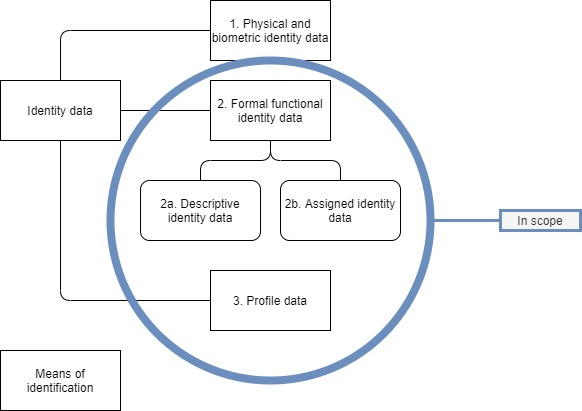
\includegraphics[width=10cm]{Identity data defintions and domain-Overview.jpg}\\
\caption{De Vries \etal - Domain of Identity Data.}
\label{fig:ID_domain}
\end{figure}
\begin{enumerate}
\item \textit{Physical and bio-metric identity data} - General physically identification data. For example, sex, height, hair color, iris, DNA-profile or medical history
\item \textit{Formal functional identity data} - Data assigned or ascribed in a certain stage of phase of life. To functionally distinguish individuals and assign rights and obligations to this individual.
\begin{enumerate}
\item \textit{Descriptive identity data} - Data that describes a person and the persons surroundings. Information that is close to the individual and is factual and mostly static. For example, family-name, parents, Place, date and time of birth. 
\item \textit{Assigned identity data} - Data that is assigned and mostly describes a (contractual) relationship with organisations to provide products and services.
\end{enumerate}
\item \textit{Profile data} - Based on a certain set of factual data, an algorithm defines profiles that categorize a person. 
\end{enumerate}

\subsection{Definition of Identity Fraud - scoped at Identity theft for this research}
While executing this research it became clear that identity Fraud is a catch-all term. De Vries \etal \cite{97408536fd1c4f4e9d1615b7a4a4473e} have analysed 30 international definitions and formulated a general description "Identity Fraud is to obtain, to possess or to create intentionally, (and) (unlawfully or without consent) false means of identification
in order to commit unlawful behaviour, or to have the intention to commit unlawful behaviour." In the footnote it states: "It must be noted that ‘false’ in the description refers to the idea that the means of identification do not identify the person who uses them truthfully." It's needed to say this is a generic definition. Figure \ref{fig:ID_fraud} shows the different types of mismatch between a person and identity data, defined by De Vries \etal \cite{Vries2007IdentiteitsfraudeEA}. This research will focus on a subset of Identity Fraud, namely Identity Theft.
\graphicspath{ {./images/} }
\begin{figure}
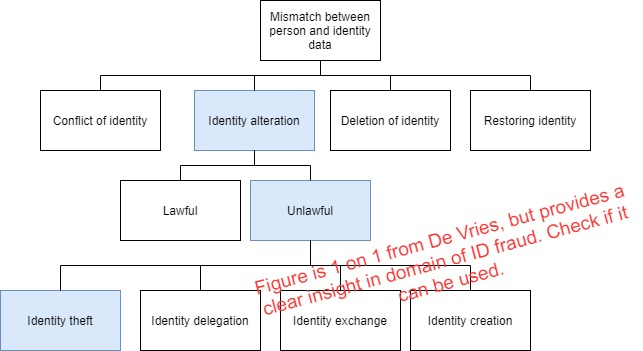
\includegraphics[width=10cm]{Domain of Identity fraud.jpg}\\
\caption{Domain of Identity Fraud}
\label{fig:ID_fraud}
\end{figure}

\subsection{Quantitative impact of Identity Fraud}\label{QI}
De Vries \etal state it's difficult to quantify identity fraud, because it's incorporated in other crimes.\cite{Vries2007IdentiteitsfraudeEA}. Goudriaan \etal claim many crimes in Western countries are not even reported to the police \cite{Gourdriaan_etal}. Quantification is relevant to define how vast a problem is and how a possible solution could mitigate it. Emphasis of this research will be logical reasoning and argumentation and not quantification of the effect of a solution. Firstly, because this is not realistic due to time restrictions. Secondly, it's needed to define an exact quantification method. Which is not the scope of this research. However, even if quantified correctly, selected countermeasures would only contain substantiated arguments by means of logical reasoning or extensive research after applying it.

A report of the Auditdienst Rijk (ADR)\cite{ADR} takes in account numbers of the citizen service for Identity Fraud at the National Office for Identity Data (Rijksdienst voor Identiteitsgegevens). Somewhere around 4.0000 citizens a year contact this service to report identity fraud. In some cases, the impact is low and only a discomfort. In other cases, the fraud results in identity theft that can lead, for example, to debts or fines.\par

However, over time Statistics Netherlands (CBS) quantified data of identity fraud, based on statistical data. Purely looking at the data classified by Identity Fraud, CBS defines it: "Without permission, via internet, making usage of someones personal data for financial gain, for example by withdraw or transfer of money, take out a loan or request of official documents." Roughly 0.5\% of Dutch citizens in 2019 became victim of identity fraud. Based on a population of 17 million, this means roughly 86.000 people are confronted with Identity Fraud each year. 
\todo{TABEL HIER "https://opendata.cbs.nl/#/CBS/nl/dataset/82464NED/table?ts=1637054627124"
"https://opendata.cbs.nl/#/CBS/nl/dataset/82464NED/barh?ts=1637054521497"
"https://opendata.cbs.nl/#/CBS/nl/dataset/82464NED/table?ts=1637054352194"}.
When looking at a broader scope, to anticipate on a definition creep, another research of the CBS is relevant {\cite{CBS_casualtiesDigitalCrime}} and zooms in on the way casualties act.

\subsection{Role of the UIN}
The World Bank \cite{WorldBank_UIN} defines ID numbers "In the context of foundational systems, ID numbers are considered to be “unique when: firstly, the number-generating process ensures that no two people within the system share the same number and secondly, a deduplication process ensures that the same person does not have multiple identity records or numbers (i.e., that they are unique in the database)." The World Bank identifies two derived strengths, namely ‘Uniqueness and deduplication’ and ‘Data matching and interoperability’. This means each person can be identified uniquely, allowing for a fast and easy exchange of identity related information between different organizations.\par 
However, the benefit of fast and easy exchange of identity related information, is also highly susceptible to misuse. Identity Fraud and Theft leans heavily on the benefit of ‘Data matching and interoperability’ of the UIN. A second form of misuse that leans on this benefit is Unauthorized data correlation. \par

\subsection{Personal Records Database (BRP) and data provisioning}\label{BRP}
The Dutch Personal Records Database or Basisregistratie Personen (BRP) contains personal information (including BSN) and history of a person in a list of attributes. BRP contains the person lists of both residents and non-resident. Residents are citizens residing in a municipality for a consecutive period. Non-residents are citizens with Dutch nationality who live abroad or people temporarily living or working within The Netherlands. \cite{BRP} The BRP provides a selection of attributes or a complete person list of all attributes to organizations which are permitted by law. After providing information, the receiving organization replicates the personal information to it's own database. From a data minimization perspective the provided content of information is minimized for the purpose of use.  
Providing and replicating a set of data is designed and implemented with the historical perspective of limitations on bandwidth and systems based on batch processing. Currently, bandwidth and real-time processing are not mentioned as concerns by interviewees or consulted experts. It could be considered as a power consumption consideration, but not defined as a quality requirement within this research.

\subsection{Operational problem}\label{OP}
The World Bank ID4ID defines vulnerabilities and risks when UINs are ubiquitous available \cite{WorldBank_protecting}. Identity theft and fraud and unauthorized data correlation are two operational problems. This research will focus on the practical problem of unauthorized correlation, in section \ref{Identity_datatypes} defined as 'Profile data', by using 'Formal functional identity data'. The UIN of a person can be defined as 'Assigned identity data'. Architectural patterns and tactics will focus on mitigating this problem, taking relevant QA's and ASRs into account. 
The UK national fraud and cybercrime reporting centre states only a name, date of birth and current or previous addresses is needed to commit identity fraud. \cite{Action_fraud}
Identity data can be obtained by personal data in a data breach, for example a breach via commercial parties or (semi-)government. Recent examples are Booking.com \cite{Booking_databreach} or the Dutch GGD \cite{GGD_databreach}.
Concretely, providing and replicating identity information could result in unforeseen misuse. Applying patterns to minimize provided data but still providing the lawfully mandated data sharing of BRP could mitigate this risk.
%Dutch laws enforce the exchange of identity data of a citizen and explicitly state to include BSN in this dataset. These laws exist in order to stimulate controlled exchange of personal data. This applies to government bodies , pension providers  and healthcare organizations. Usage of an alternative method, not explicitly providing a BSN, can be interpreted as not complying with these laws. This interpretation is not in scope for my thesis research.\par However, technologies like encryption and pseudonymisation are explicitely stated in General Data Protection Regulation (GDPR, REGULATION (EU) 2016/679) {\cite{GDPR}} to be in place as a safeguard. Other rules and regulations may apply, but are not in scope.
%
%\subsection{Pseudonymization or tokenization of a UIN}
%Researching possible solutions in literature and consulting experts showed %two viable methods worth analyzing. Pseudonymization and tokenization. %Pseudonymization of BSN already has been applied within the Dutch %government by Logius. Previous work by AuditDienst Rijk on the usage of BSN % already discussed pseudonymization as an option. Tokenization is an %alternative method largely applied in payment sector (Adyen and Apple Pay) %to ensure privacy of customers. This method is suggested by the World Bank %as a possible solution to replace a UIN, because it’s been applied within %the governments of Austria, India and Estionia.\par
%The difference between these two techniques is mainly the method of %reversing. While pseudonymization needs a key to decrypt, the techniques %behind tokenization need a form of ledger or table to lookup the original %record.
%Off course, there are a lot more technological methods. However, the scope %of this research will not be assessing all of them, rather creating a %useful framework to assess these methods based on requirements.\par
%\textbf{Pseudonymization} 
%GDPR \cite{GDPR} defines ‘pseudonymisation’: means the processing of %personal data in such a manner that the personal data can no longer be %attributed to a specific data subject without the use of additional %information, provided that such additional information is kept separately %and is subject to technical and organisational measures to ensure that the %personal data are not attributed to an identified or identifiable natural %person; \par
%\textbf{Tokenization} is described by The World Bank  as “Tokenization can %protect privacy by ensuring that only tokens, rather than a permanent %identity number or other UIN, are exposed or stored during a transaction.” %Also, by this definition, the same person is represented by different %tokens in different databases. A fundamental property, besides it’s unique %character, is it’s not possible to reverse engineer a person’s identity, %because the unique token does not contain this data.\par
%The World Bank defines two primary types of tokenization. Firstly, %\textbf{Front-end tokenization} is the creation of a token by the user as %part of an online service that can later be used in digital transactions in %place of the original identifier value. Secondly, in case of %\textbf{Back-end tokenization} the identity provider (or token provider) %tokenizes identifiers before they are shared with other systems, limiting %the propagation of the original identifier and controlling the correlation %of data. Back-end tokenization is done automatically by the system without %user intervention, meaning that people do not need to do anything manually %or understand why they would need to create tokens, eliminating any %potential digital divide and protecting identifiers and UIN at source.”